\documentclass[10pt,a4paper,titlepage]{article}
\usepackage{latexsym}
\usepackage[a4paper,top=2.5cm,bottom=2.5cm,left=2.5cm,right=2.5cm]{geometry}
\usepackage[utf8x]{inputenc}
\usepackage{booktabs,caption,amsfonts,amssymb,fancyhdr, amsmath}
\usepackage[english]{babel}
\usepackage{indentfirst}
\usepackage{multirow}
\usepackage{float}
\renewcommand*{\familydefault}{\sfdefault}
\usepackage{graphicx}
\usepackage{hyperref}
\usepackage{color}
\usepackage{amsmath}
\usepackage[squaren, Gray, cdot]{SIunits}
\usepackage{subcaption}
\usepackage{listings}
\usepackage{lipsum}


\lstset{language=c++}
\lstset{backgroundcolor=\color{white}}
\lstset{frame=single}
\lstset{stringstyle=\ttfamily}
\lstset{keywordstyle=\color{red}\bfseries}
\lstset{commentstyle=\itshape\color{blue}}

\captionsetup[table]{position=top}
\addtolength{\textwidth}{1cm}
\addtolength{\hoffset}{-1cm}
\pagestyle{headings}
\begin{document}
\title{PROGETTO 5}
\begin{center}
{\LARGE \bfseries Computational Physics\par}
\vspace{0.5cm}
{\LARGE \bfseries Project 5 - Molecular Dynamics \par}
\end{center}

\vspace{1cm}

\begin{tabular*}{\textwidth}{@{}l@{\extracolsep{\fill}}l@{}}
Academic year 2015-2016	 &Team group: \\
						&Giulio Isacchini\\
                        &Giovanni Pederiva\\
                        &Alessio Pizzini\\
                        &Mattia Ubertini\\
                                           
\end{tabular*}
\begin{center}
\hrule height 2 pt
\end{center}
\section*{Abstract}
\noindent The aim of this project is to implement molecular dynamics algorithm to analyze the behavior of thermodynamical properties of argon. We have chosen a noble gas to avoid covalent bonds between atoms. The system has been initialized as a lattice made of face-centered cubic cells, since this is the geometric structure assumed by crystalline solid argon. The number of atoms considered was between $10^2$ and $10^6$. 
\\
We have simulated the time evolution of the system for different temperatures, sampling at the same time some thermodynamical properties such as temperature, energy and momentum. We have also studied the behavior of the systems depending on its density. Finally, we have implemented Berendsen thermostat.
\section*{Introduction}
\paragraph*{What is MD?}
\noindent The molecular dynamics simulation are widely used nowadays almost in every field of science from biochemistry, material science to biophysics. Molecular dynamics is a computational simulation usually applied to a complex system to study its physical properties. It is used to examine and study the dynamics of a system that can't be directly observed experimentally.
\\
\noindent In general given a system composed by $N$ interacting components, which can be particles, atoms, molecules etc., and the interactions expression, the computer can numerically solve the $N$-coupled differential equation of Newton, which can't be solved analytically. Once the differential equation is solved, the time evolution of the system in space is obtained. Other physical properties of the system can be sampled at the same time. 
\\
\noindent In a way this can be regarded as a simulated experiment. For example this technique is used to study the dynamics of atomic level phenomena, such as film growth, which cannot be directly observed. It's widely used in biophysics to simulate the motions of the proteins and other macro molecules, in order to explain the results of biophysical experiments and modeling the interaction with other molecules.
\\  
\noindent However the problem with the numerical simulations is that they bring cumulative errors due to the numerical integration, which gets bigger at each time step. The error can be in part minimized by the usage of proper algorithms but it can't be avoided completely.  

\paragraph*{Thermodynamical assumptions}
\noindent The argon atoms were given an initial velocity according to the Maxwell distribution: 
\begin {equation}
P(v_i){v_i} = \left(\frac{m}{2\pi k_B T}\right)^{1/2} \exp\left(-\frac{m v_i^2}{2k_B T}\right) {v_i}
\end{equation}
where $m$ is the mass of the atom, $k_B$ is Boltzmann's constant and $T$ is the temperature.
\\The atoms are assumed to interact via the Lennard-Jones potential, namely:
\begin{equation}
U(r_{ij}) = 4\epsilon\left[\left(\frac{\sigma}{r_{ij}}\right)^{12} - \left(\frac{\sigma}{r_{ij}}\right)^6\right]
\end{equation}
where $r_{ij}$ is the modulus of the distance between the two atoms labelled with $i$ and $j$, $\epsilon$ and $\sigma$ are constants depending on the atom. For argon, they are: $\frac{\epsilon}{k_{B}} = 119.8 K$, $\sigma = 3.405 \angstrom$. In this potential (also known as 6-12 potential) the first term, scaling as $r^{-12}$ models Pauli repulsion between the electron orbitals, while the second one, scaling as $r^{-6}$ models van der Waals force. 
\\The total energy of the system is the sum of this potential over all the atom pairs, counting each pair once.
\ The force acting on one atom is equal to the negative gradient of the potential: 
\begin{equation}
\vec F(r_{ij}) = -\nabla U(r_{ij})
\end{equation}
so the $k$-component reads:
\begin{equation}
F_k(r_{ij}) = -\frac{\partial U}{\partial r_{ij}}\frac{\partial r_{ij}}{\partial k_{ij}}
\end{equation}
\section*{Implementation}
\noindent \paragraph{FCC Lattice} Initially, we set the particles in a cubic close-packed structure because this is the real crystal structure of solid argon. So, our lattice was made of face-centered cubic ($FCC$) unit cells of size $b$ $[\angstrom]$, which is the lattice constant. Each cell contained 4 particles in the following positions: 
\begin{equation}
\begin{split}
\vec r_1 &= 0 \hat{\textbf{i}} + 0 \hat{\textbf{j}} + 0 \hat{\textbf{k}},\\
	\vec r_2 &= \frac{b}{2}  \hat{\textbf{i}} + \frac{b}{2} \hat{\textbf{j}} + 0 \hat{\textbf{k}},\\
	\vec r_3 &= 0 \hat{\textbf{i}} + \frac{b}{2} \hat{\textbf{j}} + \frac{b}{2} \hat{\textbf{k}},\\
	\vec r_4 &= \frac{b}{2} \hat{\textbf{i}} + 0 \hat{\textbf{j}} + \frac{b}{2} \hat{\textbf{k}} 
    \end{split}
\end{equation}
where $\hat{\textbf{i}}, \hat{\textbf{j}}, \hat{\textbf{k}}$ are three orthonormal vectors. The origin of the other cells had to be set at an integer number of cell lengths from the origin:
\begin{equation}
\vec R_{i,j,k} = ib \hat{\textbf{i}} + jb \hat{\textbf{j}} + kb \hat{\textbf{k}}
\end{equation}
where $i,j,k$ are integers.
\\The lattice constant $b$ was initially set at $5.26 \angstrom$, which is the real unit cell size in argon crystals. The mass density resulted to be $1823 \frac{kg}{m^3}$. This density is extremely high when the argon is in a fluid state, since the critical density is at about $536 \frac{kg}{m^3}$.
\\After having initialized the particles positions and initial velocities (the latter according to Maxwell distribution eq.(1)), we computed the total momentum of the system and we subtracted to every atom the mean velocity, so now the total momentum in equal to zero.
\paragraph{Interactions Forces} The forces were computed according to eq.(4),  simply computing both partial derivatives analytically from eq. (2) and the trivial equation $r=\sqrt{x^2+y^2+z^2}$: 
\begin{equation}
\frac{\partial U}{\partial r_{ij}}= 4\epsilon\left[-12\left(\frac{\sigma^{12}}{r_{ij}^{13}}\right) + 6\left(\frac{\sigma^{6}}{r_{ij}^7}\right)\right]
\end{equation}
\begin{equation}
\frac{\partial r_{ij}}{\partial k_{ij}} = \frac{k_{ij}}{r_{ij}}
\end{equation}
\\Since the number of couple particles is $\frac{N^2}{2}$, and the number of particles $N$ scales as four times the cube of the number of unit cells per edge of the lattice, so the number of calculations increased sharply as the lattice dimension increased. To reduce the elapsed time, once computed the distance between two particles we ignored their interaction if they are separated by more than 5 $\sigma$. This simplification doesn't affect the results in a noticeable way since the strength of the Lennard-Jones force decreases quickly as the distance grows as can be seen in the following graph:
\begin{figure}[H]
\begin{center}
    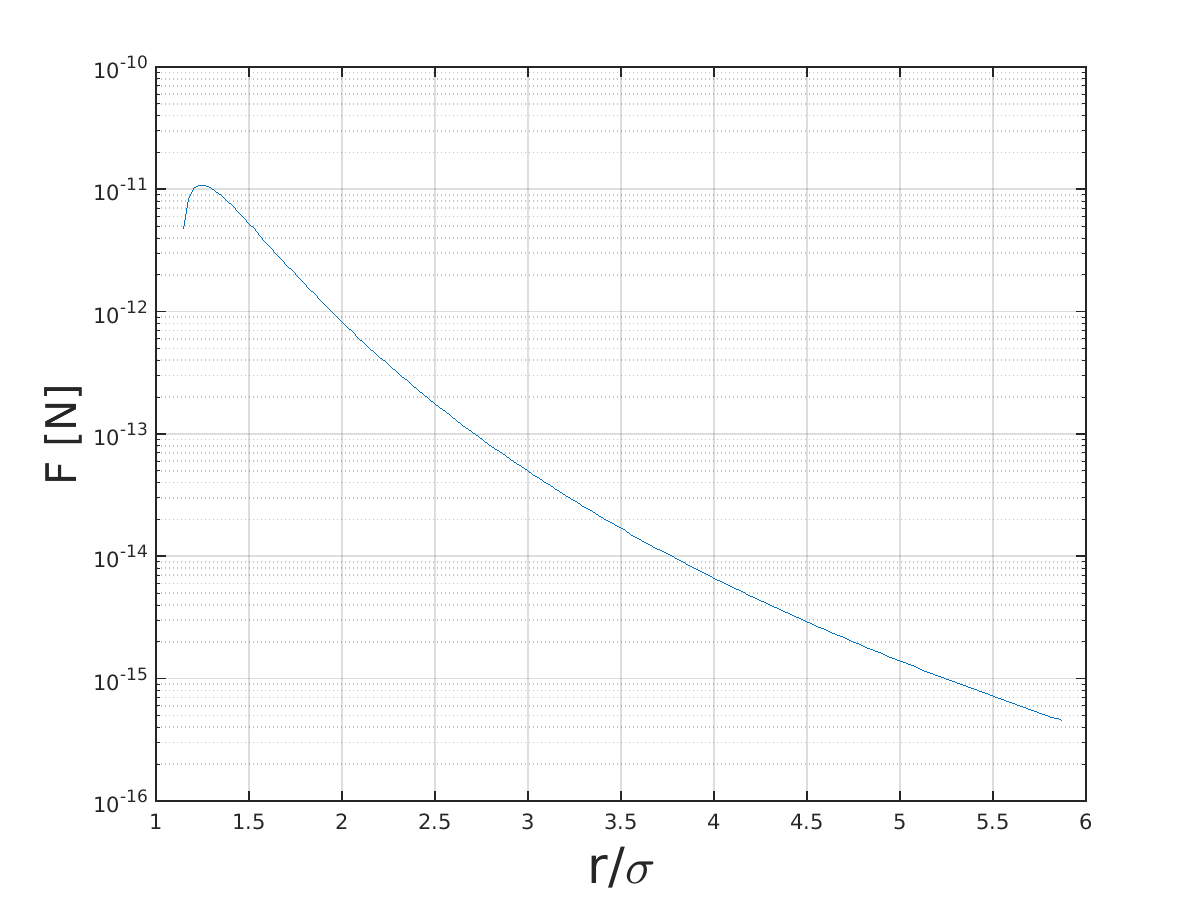
\includegraphics[width=0.4\textwidth]{forza.png}
\caption{Force between two atoms over their normalized distance. Since the y-axis is logarithmic, negative values (i.e. attractive forces) aren't plotted. The value at $5\sigma$ is about $10^{-4}$ times the maximum value.}
	\end{center}
\end{figure}
\noindent \paragraph{Cell Lists} Later, we needed to simulate bigger systems to get more realistic values for the temperature, the energy and so on. The former algorithm proved to be unsatisfactory since even if it doesn't compute the forces, it requires to compute the distance for every couple of particles. To avoid this and to be able to simulate larger systems, we were suggested and helped by Anders Hafreager to implement the cell list strategy to speed up calculations. This consist in dividing the domain in cells with length bigger than the cut-off distance of the Lennard-Jones potential ($2.5\times \sigma$) and for each atom in a certain cell, considering only the atoms in the same or in the 26 neighboring cubes. Then we computed the distance between the chosen atom and the ones in the region described above and took in account only the ones within a bigger shell having radius $2.8 \times \sigma$. The position was refreshed each time step, but only the particles within the inner sphere having as radius the cut - off distance $2.5 \times \sigma$  were counted for the calculation of the forces. When the chosen atom had moved away from its initial position more than $\frac{0.3 \sigma}{2}$, which is half of the difference between the radii of the inner sphere and the outer shell, all the cell listing process is repeated for every particle. This sped up our program by a factor of $\simeq 40$ for a 10 cells lattice on the benchmark we created, but the most noticable difference is that the code has in this way a linear dependance with the number of unit cells and not cubic anymore.
\paragraph{Boundary Conditions} The implementation od boundary conditions for positions is trivial, let's focus on forces. We implemented periodic boundary conditions for the forces in the following way: for each direction $\textbf{u}$, we computed the distance between two particles $i,j$ for each component as follows: 
\begin{equation}
k_{1,2} = \begin{cases} 
k_2-k_1   & \mbox{if} -L/2 \leq k_2-k_1 \leq L/2\\ 
k_2-k_1 + L  & \mbox{if} \hspace{0.2cm} k_2-k_1 \leq -L/2\\
k_2-k_1 - L  & \mbox{if} \hspace{0.2cm} k_2-k_1 \geq L/2 \\
\end{cases}
\end{equation}
\\ Since the only forces present in the system are internal ones, the energy is conserved. Moreover, periodic boundary conditions don't allow the system to exchange any particles with the environment, so we can state that our system is a microcanonical ensemble. Periodic boundary conditions also allow us to simulate an infinite-sized system with a limited amount of calculations. On the other hand, these boundary conditions result into more calculations since we need one or two if-tests per dimension per particle to be performed.  
\paragraph{Integrators} To refresh position and velocity of the particles, we implemented Verlet algorithm, which runs as follows:
\begin{equation}
\vec v(t + \Delta t/2) = \vec v(t) + \frac{\vec F(t)}{m}\frac{\Delta t}{2}\\
\end{equation}
\begin{equation}
	\vec r(t + \Delta t) = \vec r(t) + \vec v(t + \Delta t/2)\Delta t\\
    \end{equation}
    \begin{equation}
	\vec v(t + \Delta t) = \vec v(t + \Delta t/2) + \frac{\vec F(t + \Delta t)}{m}\frac{\Delta t}{2}
\end{equation}
\\Notice that in the Verlet intergator we compute the velocity twice during one timestep $\Delta t$ and use its value computed in the middle of the timestep to compute the new position $\vec r(t+\Delta t)$, while in a simpler Euler-Cromer integrator we would have computed the velocity just once per timestep:
 \begin{equation}
	\vec v(t + \Delta t) = \vec v(t) + \frac{\vec F(t)}{m}\Delta
\end{equation}
\begin{equation}
	\vec r(t + \Delta t) = \vec r(t) + \vec v(t+\Delta t)\Delta t\\
    \end{equation}
\\This difference results in a smaller global truncation error of the position for the former algorithm, which scales as $h$, while for the latter it scales as $h^2$. On the other hand, we now have also more flops operations than before, even if they are of the same order of magnitude.
\paragraph{Thermodynamical Parameters} To study the evolution of the system and its dependence over initial conditions (cell size $b$, initial temperature), we computed several thermodynamic quantities every timestep. 
\\ The total potential energy was computed as the sum over all pairs of atoms of their interaction energy: 
\begin{equation}
V = \sum_{i>j} U(r_{ij})
\end{equation}
The total kinetic energy is defined as
\begin{equation}
\sum_{i}^{N} \frac{1}{2}m_i v_{i}^{2}
\end{equation}
and the total energy is of course the sum of the two former energies.
\\The total energy is expected to be constant over time since the system is a microcanonical ensemble, hence there aren't exchanges neither of energy nor of particles. This is therefore a test which we implemented to verify the reliability of our algorithm.
\\Another test we made was to compute the total momentum of the system, which we initially set to zero and which we expect to remain constant, since all forces are internal. \\
We also computed the temperature of the system as a function of the average kinetic energy: \begin{equation}
\langle E_k \rangle = \frac{3}{2}N_\text{atoms} k_B T
\end{equation} This value can vary from the initial temperature (which we used for the Maxwell distribution) and we have studied this phenomenon in the data analysis.
\\We also produced animated plots of the atoms with  Ovito and we noticed that as the temperature grew, the system evolved to a more chaotic one, and above a certain temperature (its melting point) it lost its crystal structure. To have an estimate of the melting temperature we computed the diffusion constant D of the system, which is defined as $\langle r^2(t) \rangle = 6Dt$. D is expected to be about zero when the system is solid and to grow steeply around its melting point. 
\paragraph{Thermostat}Finally, we implemented Berendsen thermostat, which consists on scaling all the velocities by a factor $\gamma$ defined as 
\begin{equation}
\gamma = \sqrt{1+ \frac{\Delta t}{\tau} \left (\frac{T_{bath}}{T}-1 \right) }
\end{equation}
where $\tau$ is the relaxation time and was set to $100 \times h$, $T$ is the measured temperature and $T_{bath}$ is the desired temperature.

\newpage
\section*{Code Structure}
\noindent We have been writing our code on a object oriented framework that was already prepared. The whole implementation consists in a ensamble of nested functions called by the previous one. 
First of all we use the class \textit{UnitConverter} in order to adapt the system dimensions and generalize the implementation to a wider range of physical systems.
\\
Secondly we set up the lattice by positioning every particle into the theoretical stable $FCC$ crystal structure of the Argon and give them random velocities based on the Boltzmann distribution as a function of the initial temperature. We also remove the total initial momentum by subtracting the mean initial momentum per particle from every atom.
Then we decide which kind of subclass integrator we want to use: either \textit{Euler-Cromer} integrator or the \textit{Verlet} Integrator.
We finally finished to set up the environment, it's time to start the simulation.
\\ \newline
The flow start with the \textit{step} function of the system class that, before advancing one step forward in time, calls the function \textit{integrator} of the integrator class. We already decided which integrator we want to use at the  beginning of the code. The integrator calls the function \textit{calculateForces} from the potential class, which is at the  core of our algorithm. We analitically integrated the \textit{Lennard-Jones potential} as a function of the distance $r_{ij}$. As a consequence in the function we are able to calculate by a nested for loop the total force that every particle undergoes, taking also into account the third newton law in order to speed up the code and not compute again the same quantities.
The integrator then derives the new velocities and positions based on the forces previously calculated as described in the previous sections. Note that we applied periodic boundary conditions in order to compute the forces and the positions of the particles: the atoms can't escape the lattice.
\\ \newline
A for-loop repeats the step function a certain number of times and at every time steps thermodynamic quantities of the system are calculated. All the positions of the particles can also be stored into a file and visualized with animation tools like VMD or OVITO. Here a flow chart that simplifies what we've just explained:
\begin{figure}[H]
\begin{center}
    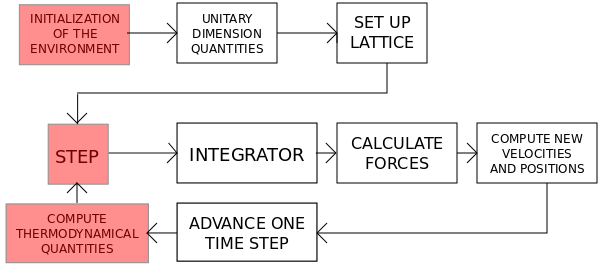
\includegraphics[width=0.8\textwidth]{FLOW.png}
\caption{Flow chart of the nested functions system}
	\end{center}
\end{figure}
\newpage
\section*{Data analysis}
\noindent We have ran our algorithm for different values of the initial (and therefore final) temperature and we then visualized the evolving system with Ovito. The first lattice we used is made of $5 \times 5 \times 5$ unit cells, corresponding to 500 atoms. The results are shown in the following graphs.
\begin{center}
\begin{figure}[H]
 \centering
\begin{subfigure}{.4\textwidth}
  \centering
  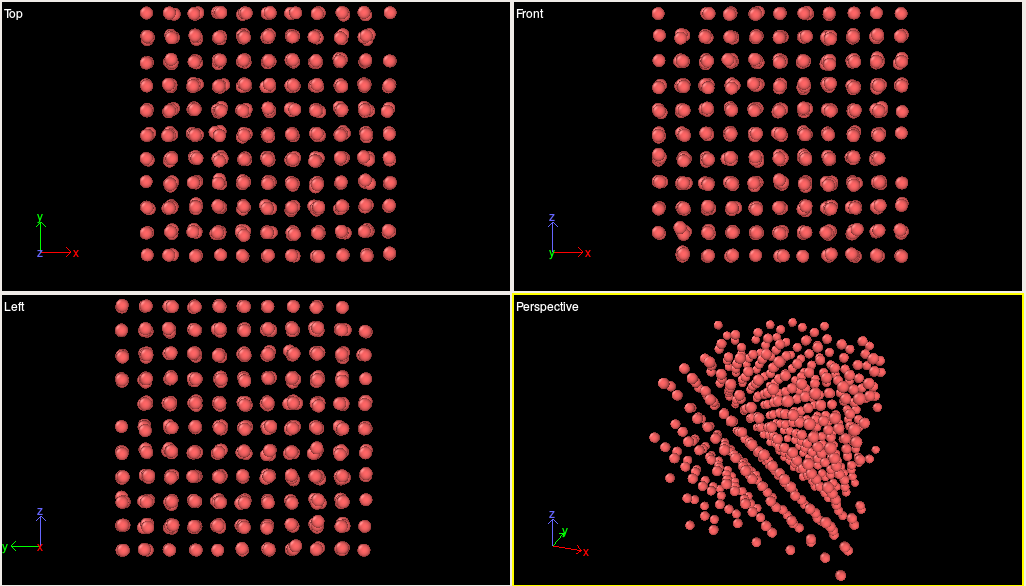
\includegraphics[width=.9\linewidth]{50.png}
  \caption{\footnotesize T = 50 K}
  \label{fig:sfig2}
\end{subfigure}%
\begin{subfigure}{.4\textwidth}
  \centering
  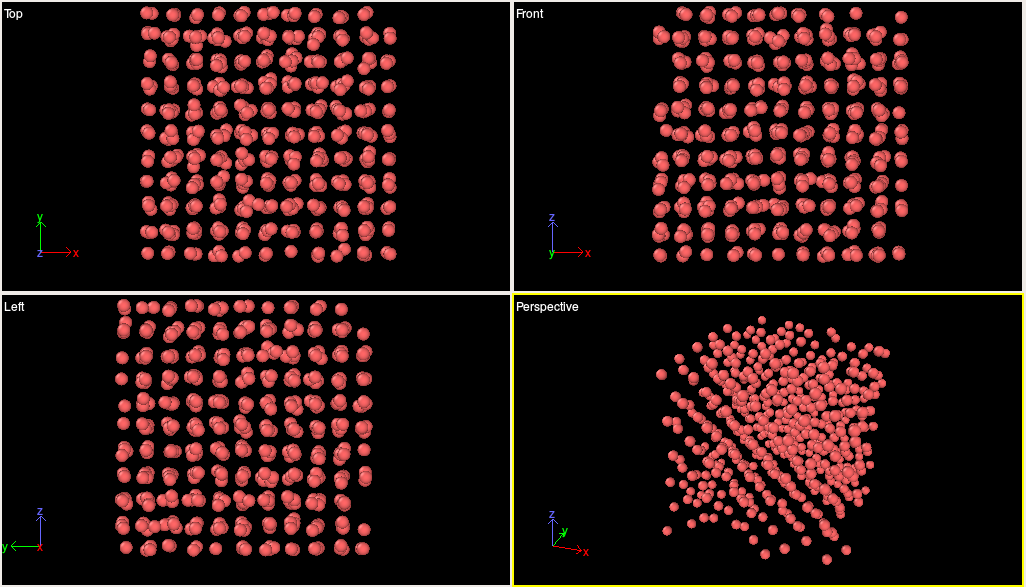
\includegraphics[width=.9\linewidth]{200.png}
  \caption{\footnotesize T = 200 K}
  \label{fig:sfig2}
\end{subfigure}
\begin{subfigure}{.4\textwidth}
  \centering
  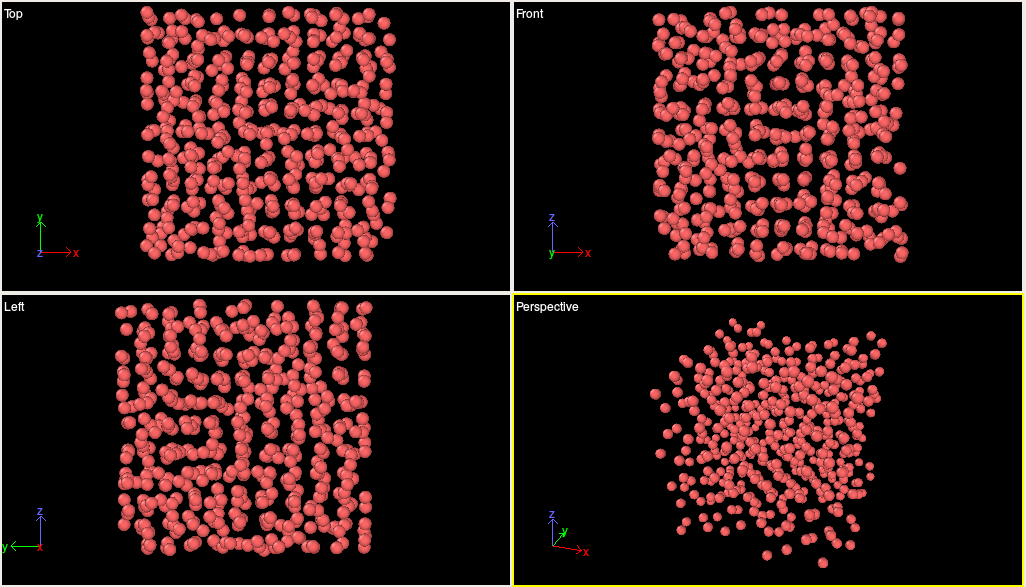
\includegraphics[width=.9\linewidth]{350.png}
  \caption{\footnotesize T = 350 K}
  \label{fig:sfig2}
\end{subfigure}%
\begin{subfigure}{.4\textwidth}
  \centering
  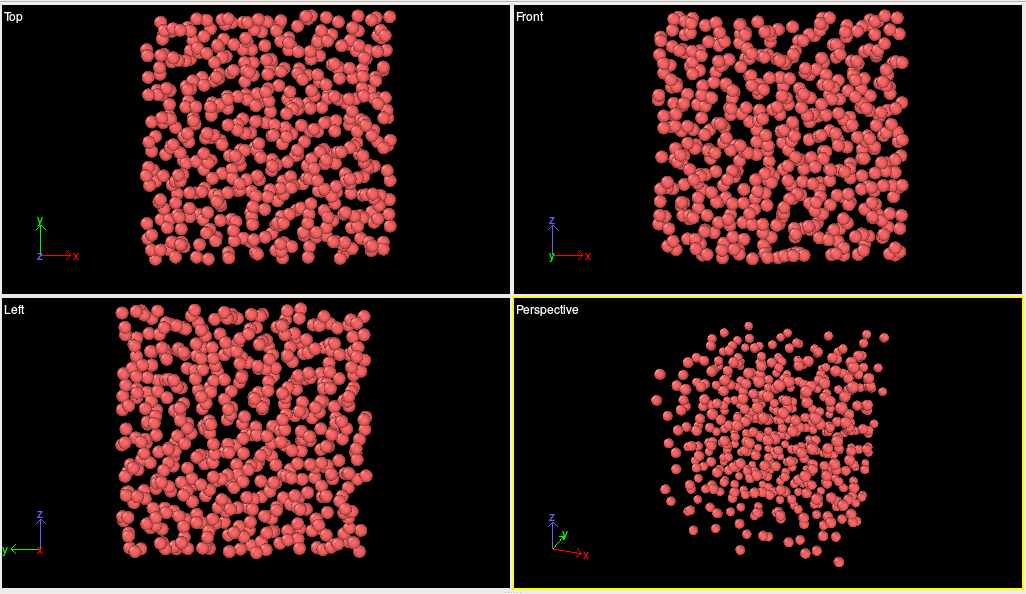
\includegraphics[width=.9\linewidth]{500.png}
  \caption{\footnotesize T = 500 K}
  \label{fig:sfig2}
\end{subfigure}%
\caption{{\footnotesize Here the final state of the system is plotted for different final temperatures. For the highest ones, the crystal structure of the system isn't present anymore. To be sure to have reached a steady state, we waited for the value of the temperature to have reached an almost constant value.}}
\label{fig:fig}
\end{figure}
\end{center} 
As expected, as temperature grows, the system becomes more chaotic and at some point (for example, see fig.3 d) the atoms aren't bonded anymore to their positions in the crystal structure and the system becomes fluid. Despite this, it is not easy to detect the exact melting point graphically, hence a new quantity was computed: the diffusion constant. It is defined as follows: $\langle r^2(t) \rangle = 6Dt$. When the structure is solid $D$ is expected to be about zero since the displacement of each atom from its initial position is negligible, while when the system melts $D$ is expected to grow sharply and then to scale as the temperature according to Einstein's relation: $D=\mu k_B T$, where $k_B$ is Boltzmann's constant, $\mu$ the mobility and $T$ the temperature. The results are shown in the following graph:
\begin{figure}[H]
\begin{center}
    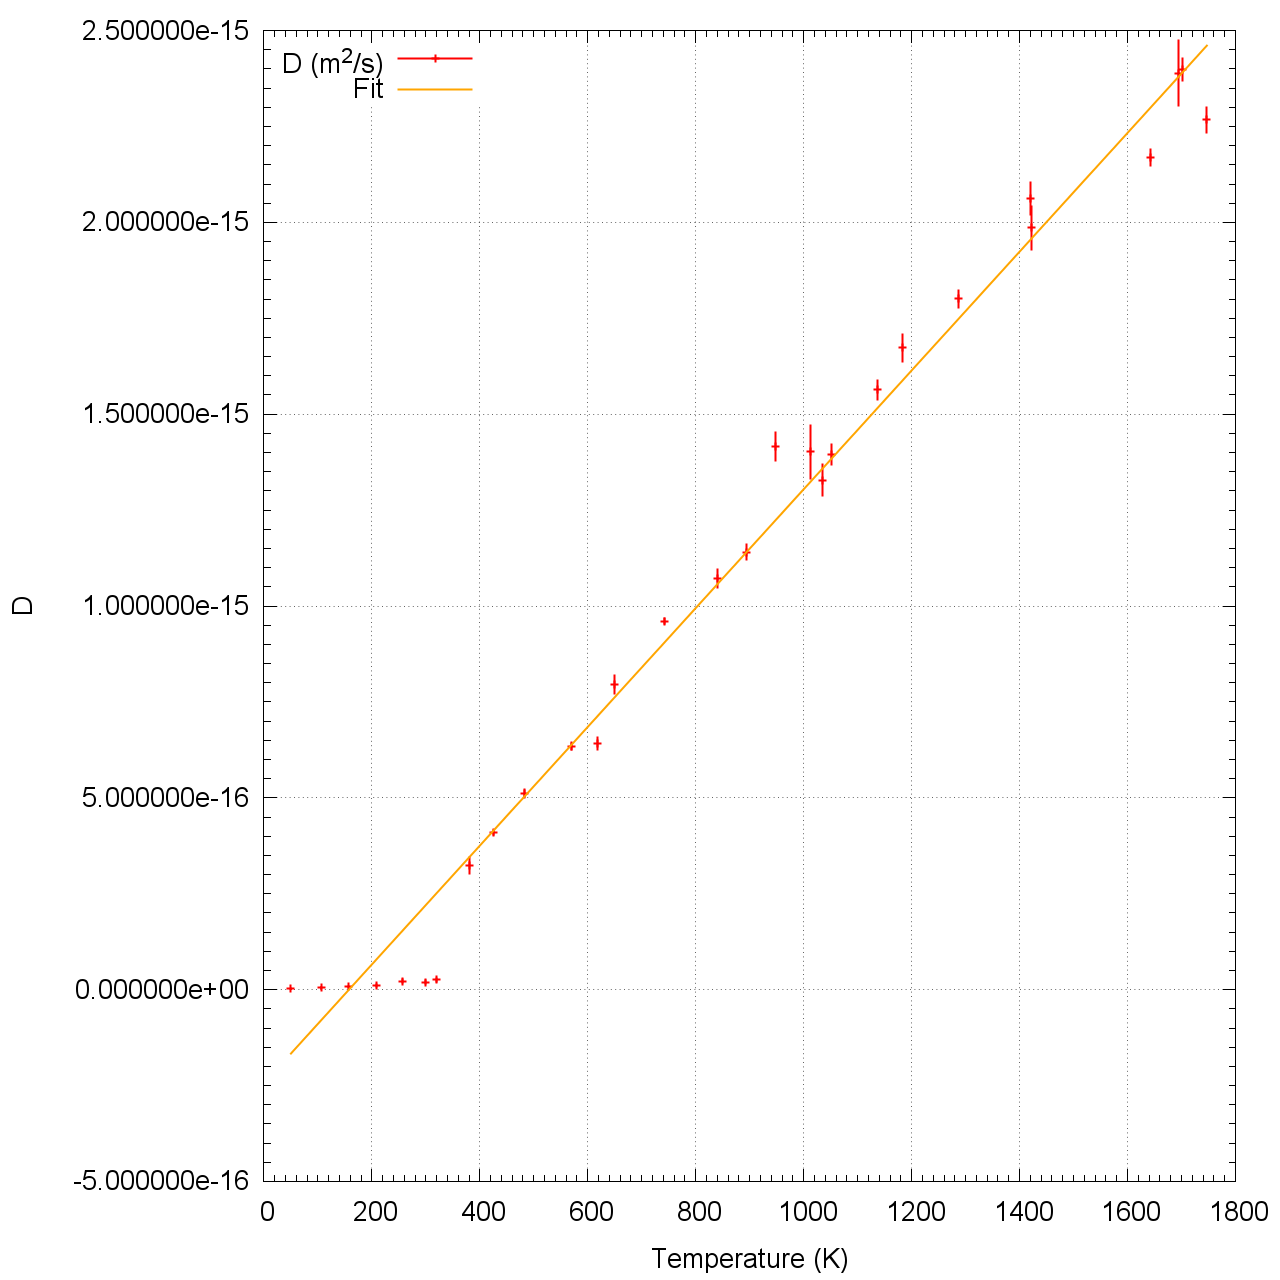
\includegraphics[width=0.4\textwidth]{plot_diffusion_temp.png}
\caption{D as a function of T, D has dimensions $[m^2 /s]$}
\end{center}
\end{figure}
\noindent As expected, $D$ is negligible for low temperatures, then it grows sharply between 340K and 380K and keeps growing linearly after. The melting temperature we found ($340 K < T_M < 380$) is much higher than the melting temperature ($84 K$) at standard conditions because in our case the density is about $10^3$ times the density at standard conditions.
\\

\noindent To be able to analyze results as function of time, we plotted the kinetic energy, the potential energy and their sum, i.e. the total energy over the number of time-steps. Here follow the results:
\begin{center}
\begin{figure}[H]
 \centering
\begin{subfigure}{.5\textwidth}
  \centering
  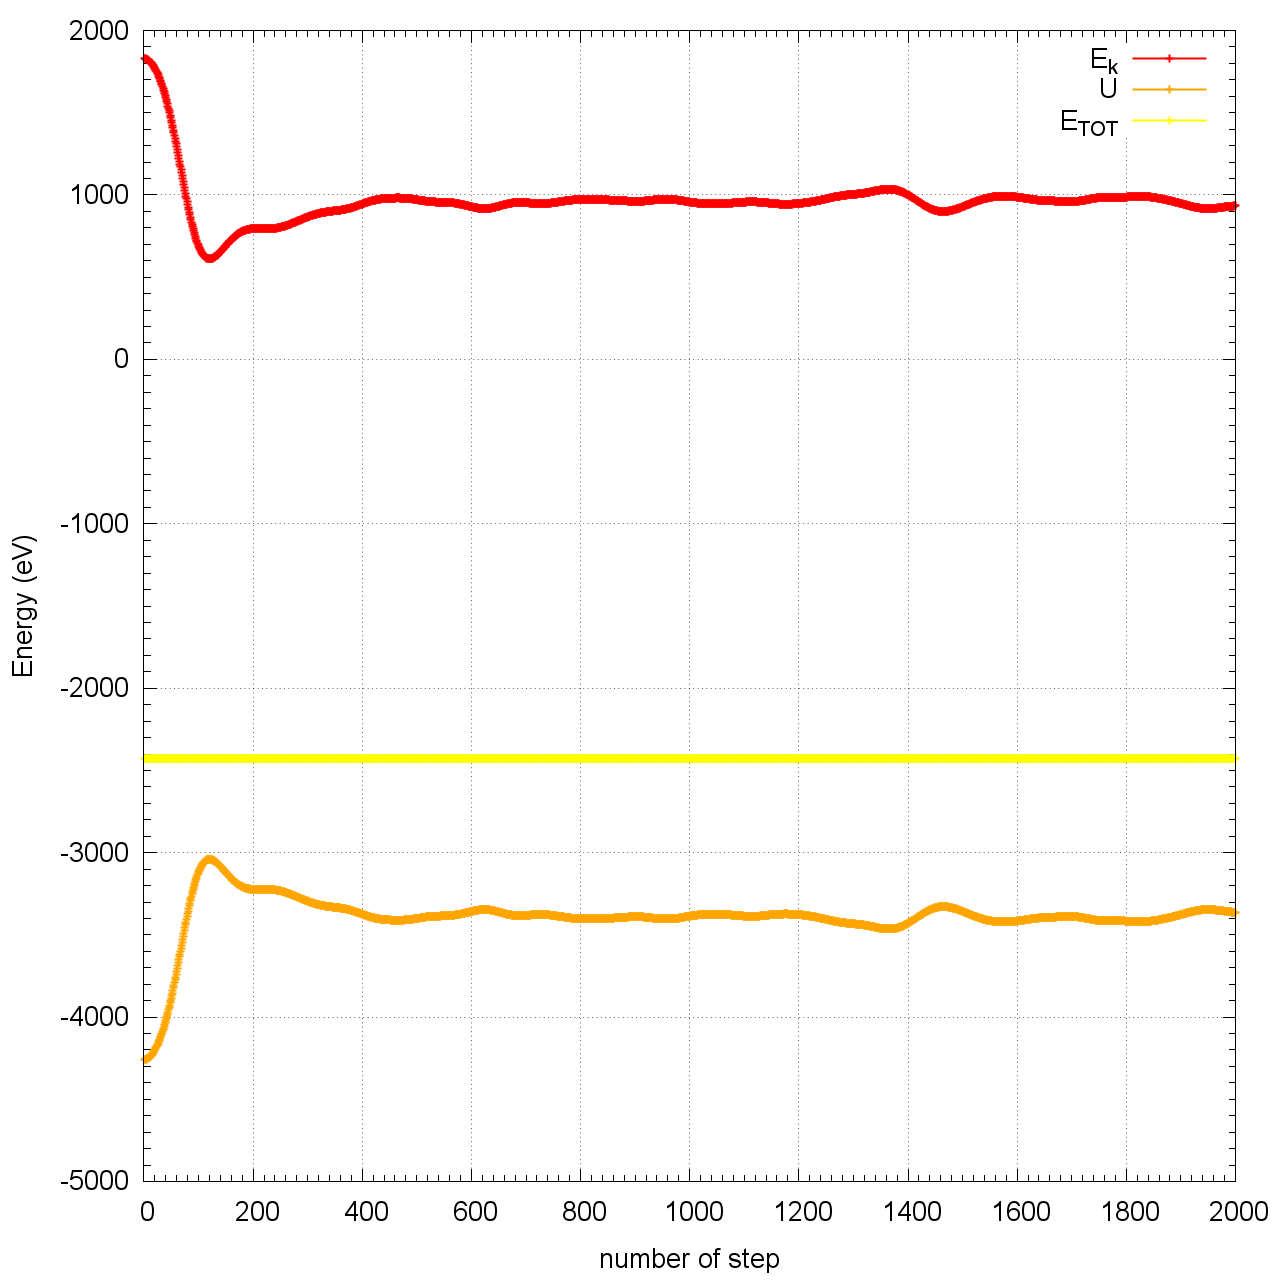
\includegraphics[width=.9\linewidth]{plot_energy_no_term.png}
  \caption{$E_k$, $E_{pot}$ and $E_{tot}$ over the number of time-steps. \\ In about 100 time-steps, the kinetic energy drops to \\ half its initial value, while the potential energy grows \\ by the same amount.}
  \label{fig:sfig2}
\end{subfigure}%
\begin{subfigure}{.5\textwidth}
  \centering
  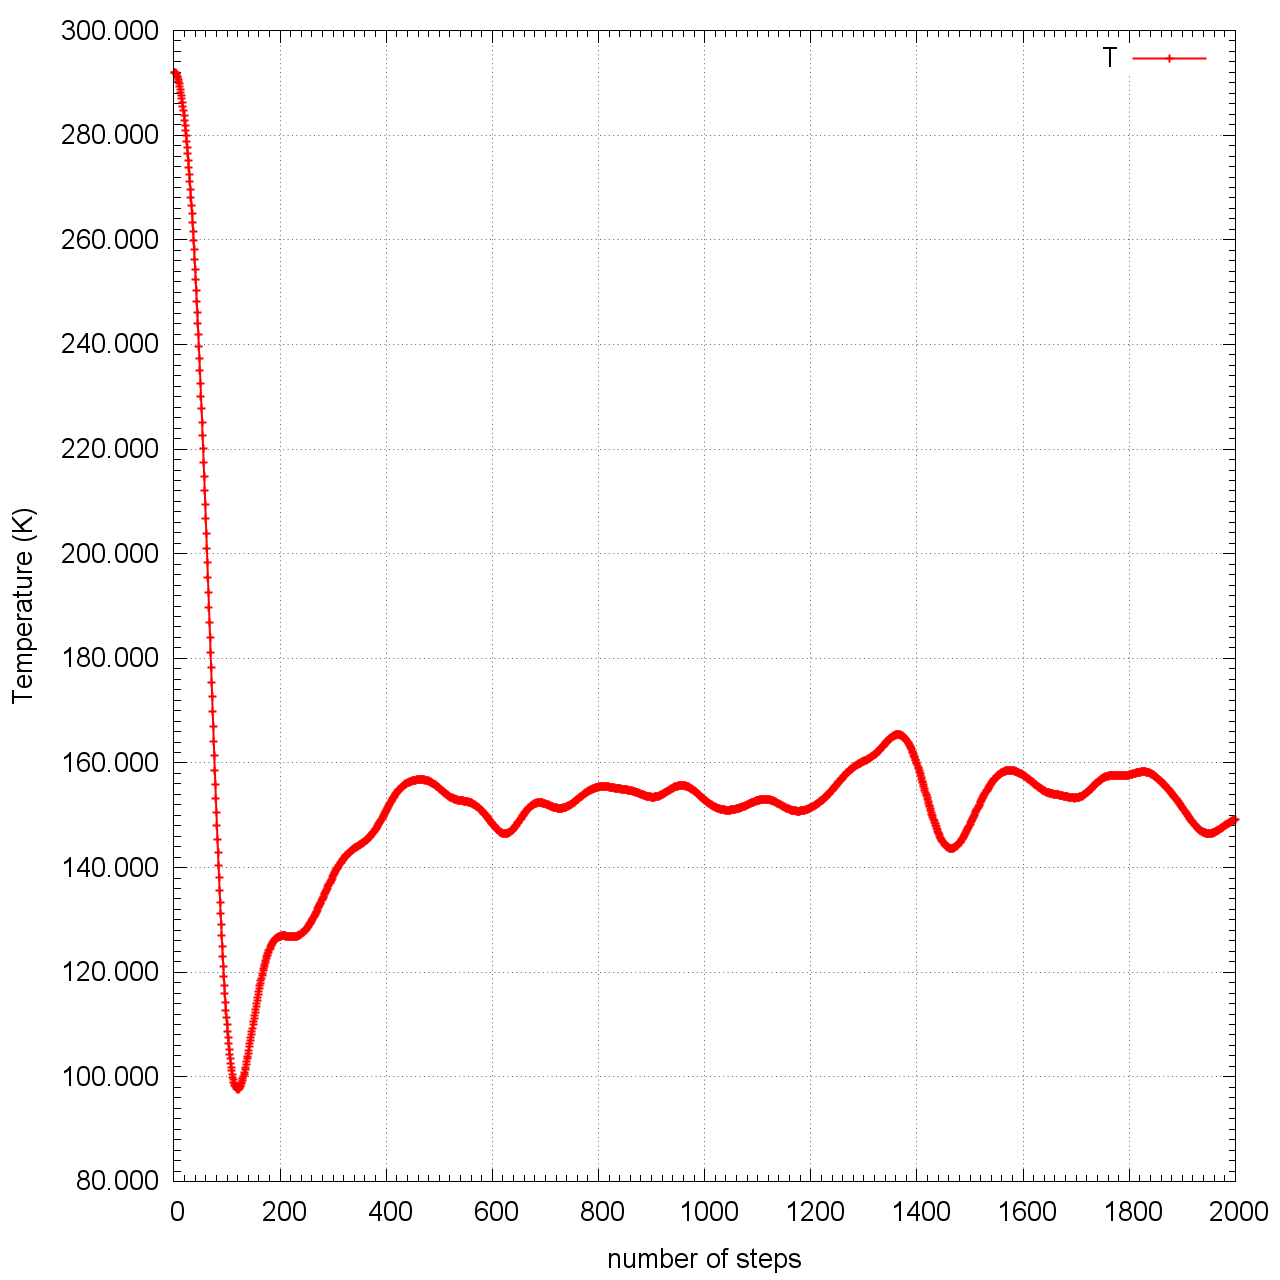
\includegraphics[width=.9\linewidth]{plot_temperature_no_term.png}
  \caption{\footnotesize Temperature over the number of timesteps. As the kinetic energy, it drops to about half its initial value.}
  \label{fig:sfig2}
\end{subfigure}%
\caption{{\footnotesize The quick growth of the potential happens because the system loses its initial ordered crystalline structure, for which the energy had a minimum. After this, the system is thermalized and the temperature (which is proportional to the kinetic energy) oscillates about a certain value, while the total energy remains constant for every time step within the first four digits, as we have expected. This is a test that shows that the algorithm is reliable.}}
\label{fig:fig}
\end{figure}
\end{center} 
\noindent At the same time we  sampled the total linear momentum of the system, starting with $P_{tot}=0 [kg \times m /s]$. Since there are not external forces we have expected that $P_{tot}$ remains constantly zero. We have verified it, in fact the sampled total linear momentum was oscillating minimally in time around  $\simeq 10^{-20} [kg \times m/s]$. 
\\
The fact, that it's not precisely zero, is due to the error brought by the integrator and round of errors. The oscillations of the energy are explained for the same reasons.
\subsection*{Evolution of initial temperature}
\noindent We ran the algorithm for different values of the initial temperature. For each case we computed the ratio between the final temperature and the initial one. Here are the results:
\begin{figure}[H]
\begin{center}
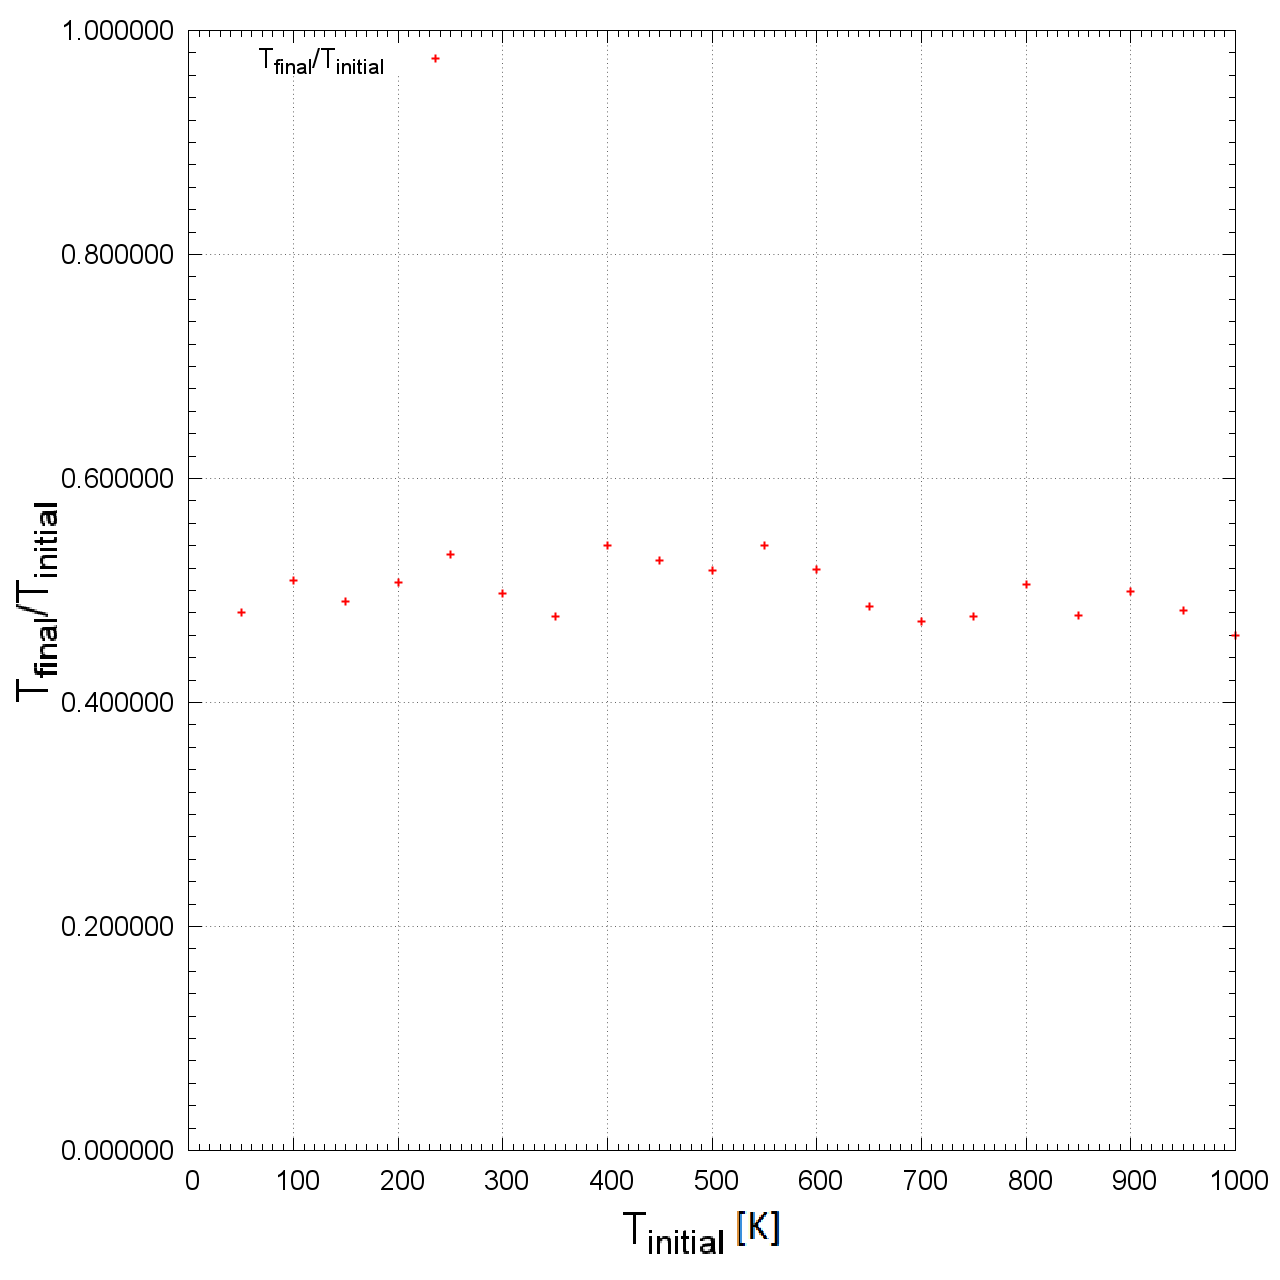
\includegraphics[width=0.4\textwidth]{plot_Tfinale.png}
\caption{The data are computed for a fixed volume, in particularly the one for which the molecules of argon are in the crystal structure. The ratio between the final temperature and the initial one is almost constant when the latter one changes and is about one half.}
\end{center}
\end{figure}
\noindent We also studied the drop of the initial temperature varying the lattice size of the system: \begin{figure}[H]
\begin{center}
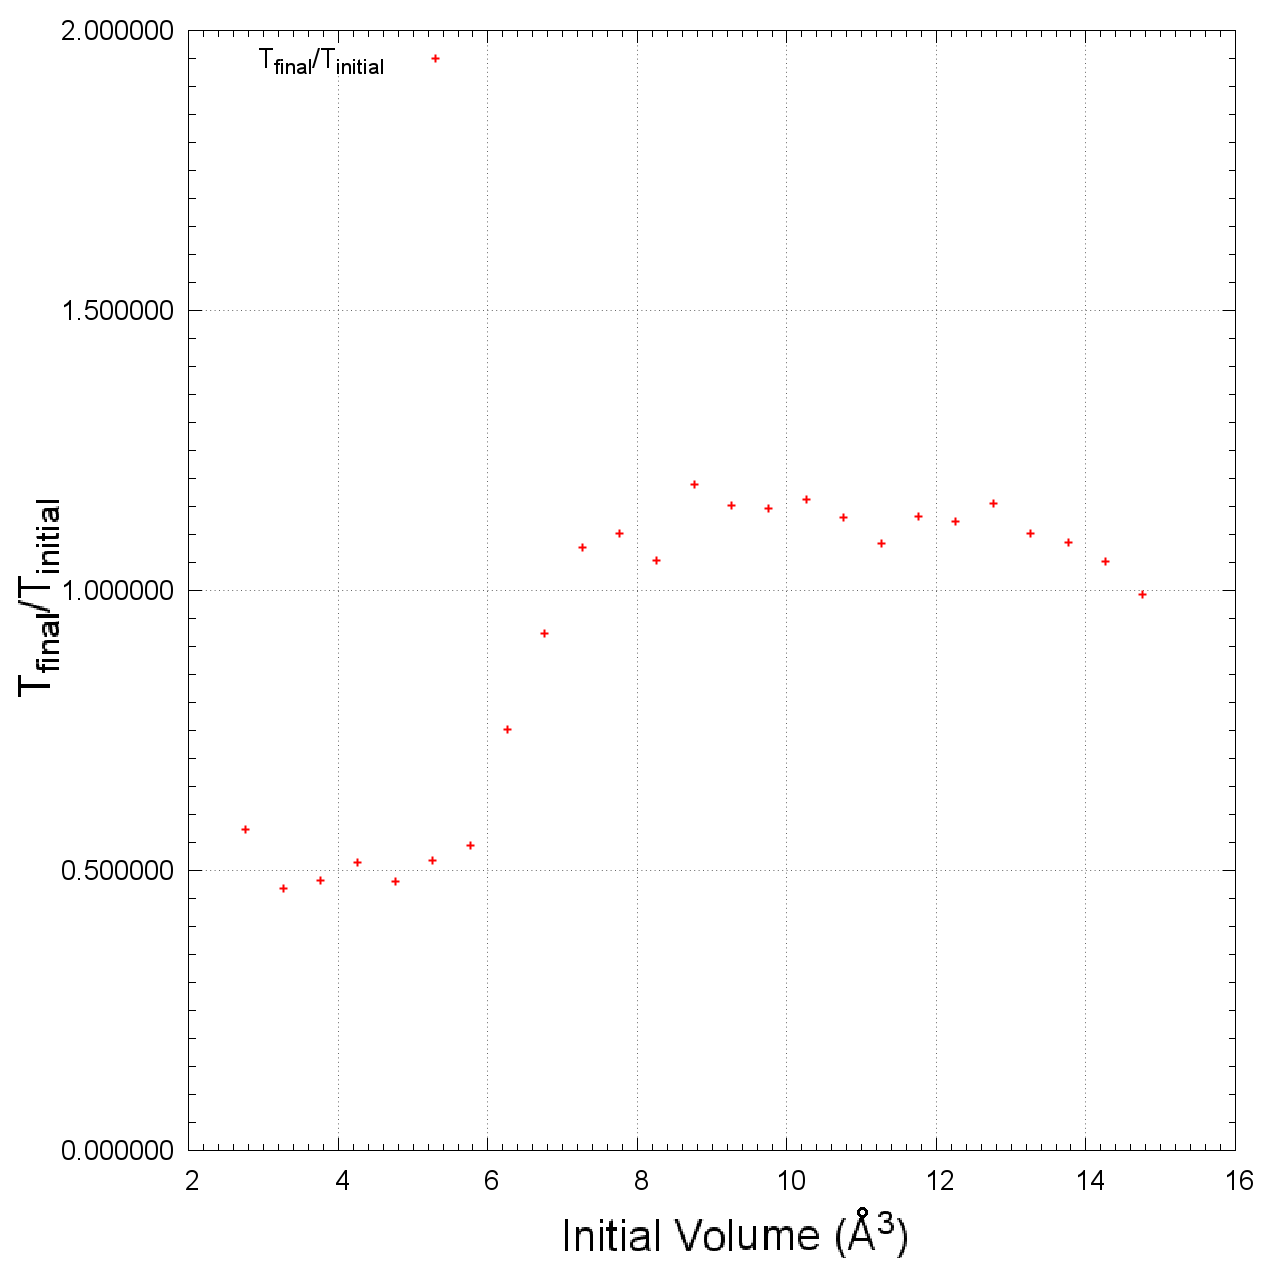
\includegraphics[width=0.4\textwidth]{plot_Tfinale_volumi.png}
\caption{The ratio between the final temperature and the initial one is almost $1/2$ for lattice size smaller than $b$,with $b$ the lattice size constant for which the crystal structure has the minimum in the potential. For lattice sizes bigger than $b$ the ratio $\frac{T_{final}}{T_0}$ gets bigger assuming also value greater than $1$ and stabilizing around this value. The fact that the ratio increases with the increasing of the lattice size is due to the fact that at this distances the initial configuration is not anymore a minimum. Hence,for the shape of the Lennard-Jones potential, the changing in the initial position of the molecules  in this configuration does not affect strongly the change on the potential and consequently the kinetic energy does not change as much as before.}
\end{center}
\end{figure} 
\subsection*{Error analysis}
\noindent Another analysis we carried had the aim to compare Euler-Cromer and Verlet integration. To do this, we plotted the error of the value of the energy for different values of the time step $\Delta t$ for both algorithms. The error was computed as the standard deviation of a series of values obtained with different random initial velocities. The results are shown in the following graph:
\begin{figure}[H]
\begin{center}
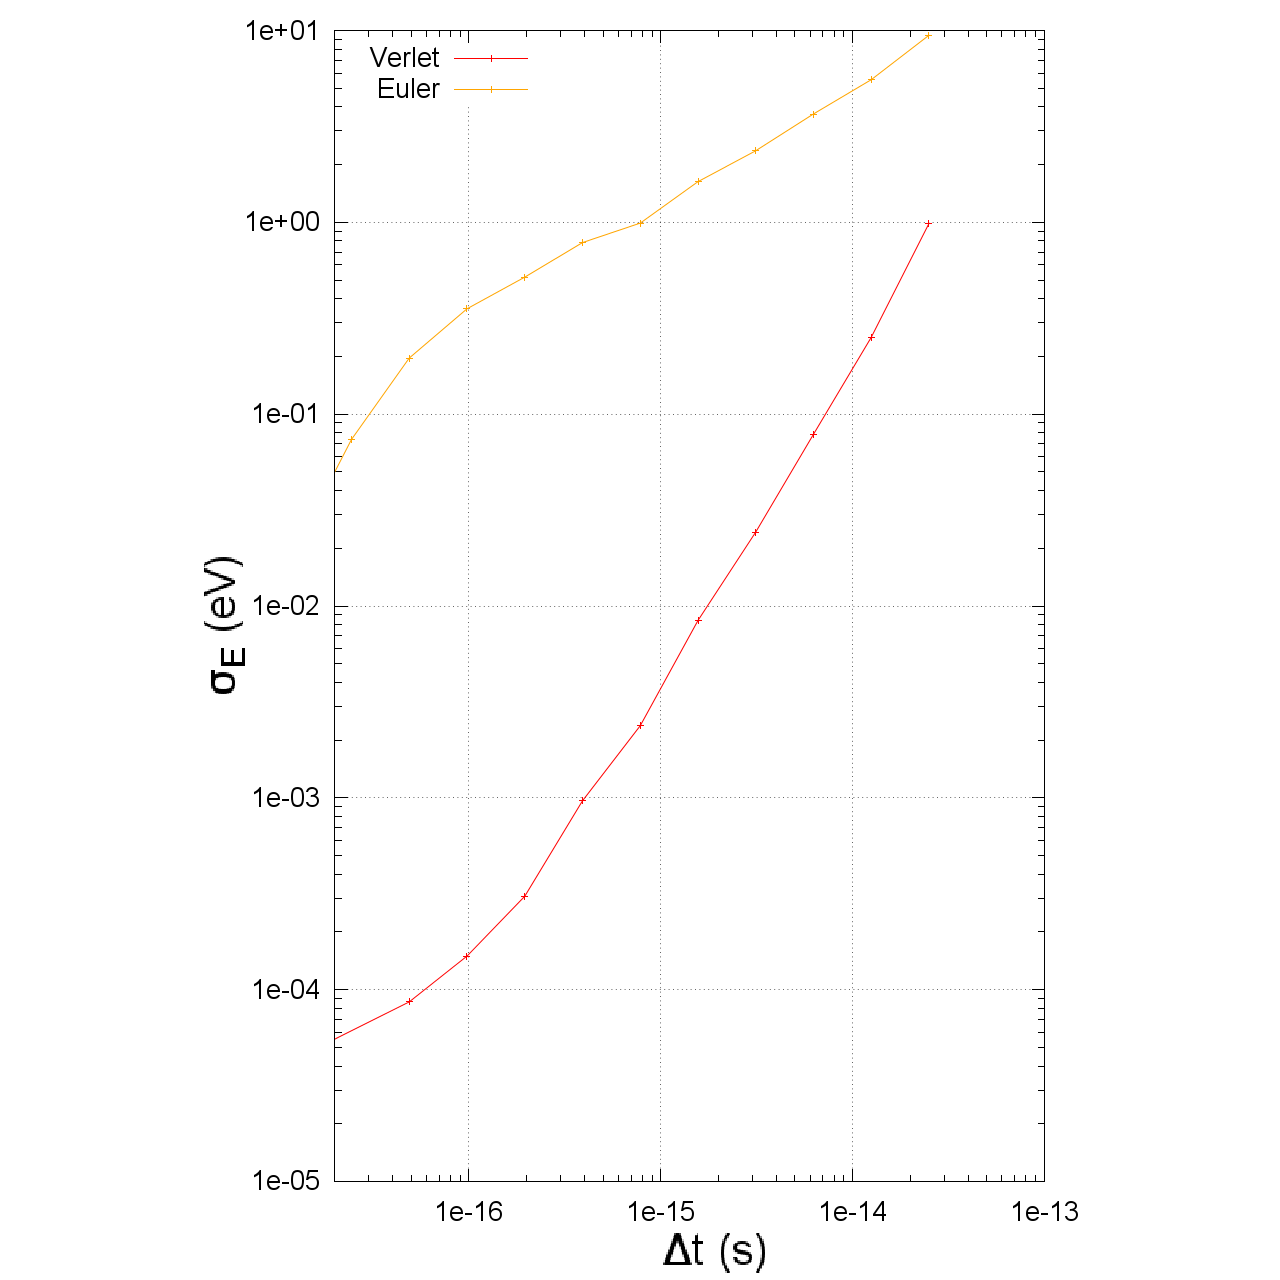
\includegraphics[width=0.4\textwidth]{plot_error.png}
\caption{The error made by the two different integration algorithms over the timestep. Verlet integration results in a smaller error.}
\end{center}
\end{figure}
\noindent As it is clearly shown the Verlet algorithm is much more accurate, as we have expected. The slope in the Verlet algorithm is about the double of the Euler-Cromer one, as it should be, since the global error for the velocity scales as $\Delta t$  for Euler-Cromer integration and as $(\Delta t)^2$ for Verlet integration. Since energy scales as $v^2$, its error should scale as $(v+\Delta v)^2 - v^2 \approx 2v\Delta v$, so it is expected to be proportional to $\Delta v$.
\subsection*{Bigger systems}\noindent 
\\We then exploited the cell list technique for a bigger lattice, made of $20 \times 20 \times 20$ unit cells, so the number of atoms was 32000. Here are the results:
\begin{center}
\begin{figure}[H]
 \centering
\begin{subfigure}{.5\textwidth}
  \centering
  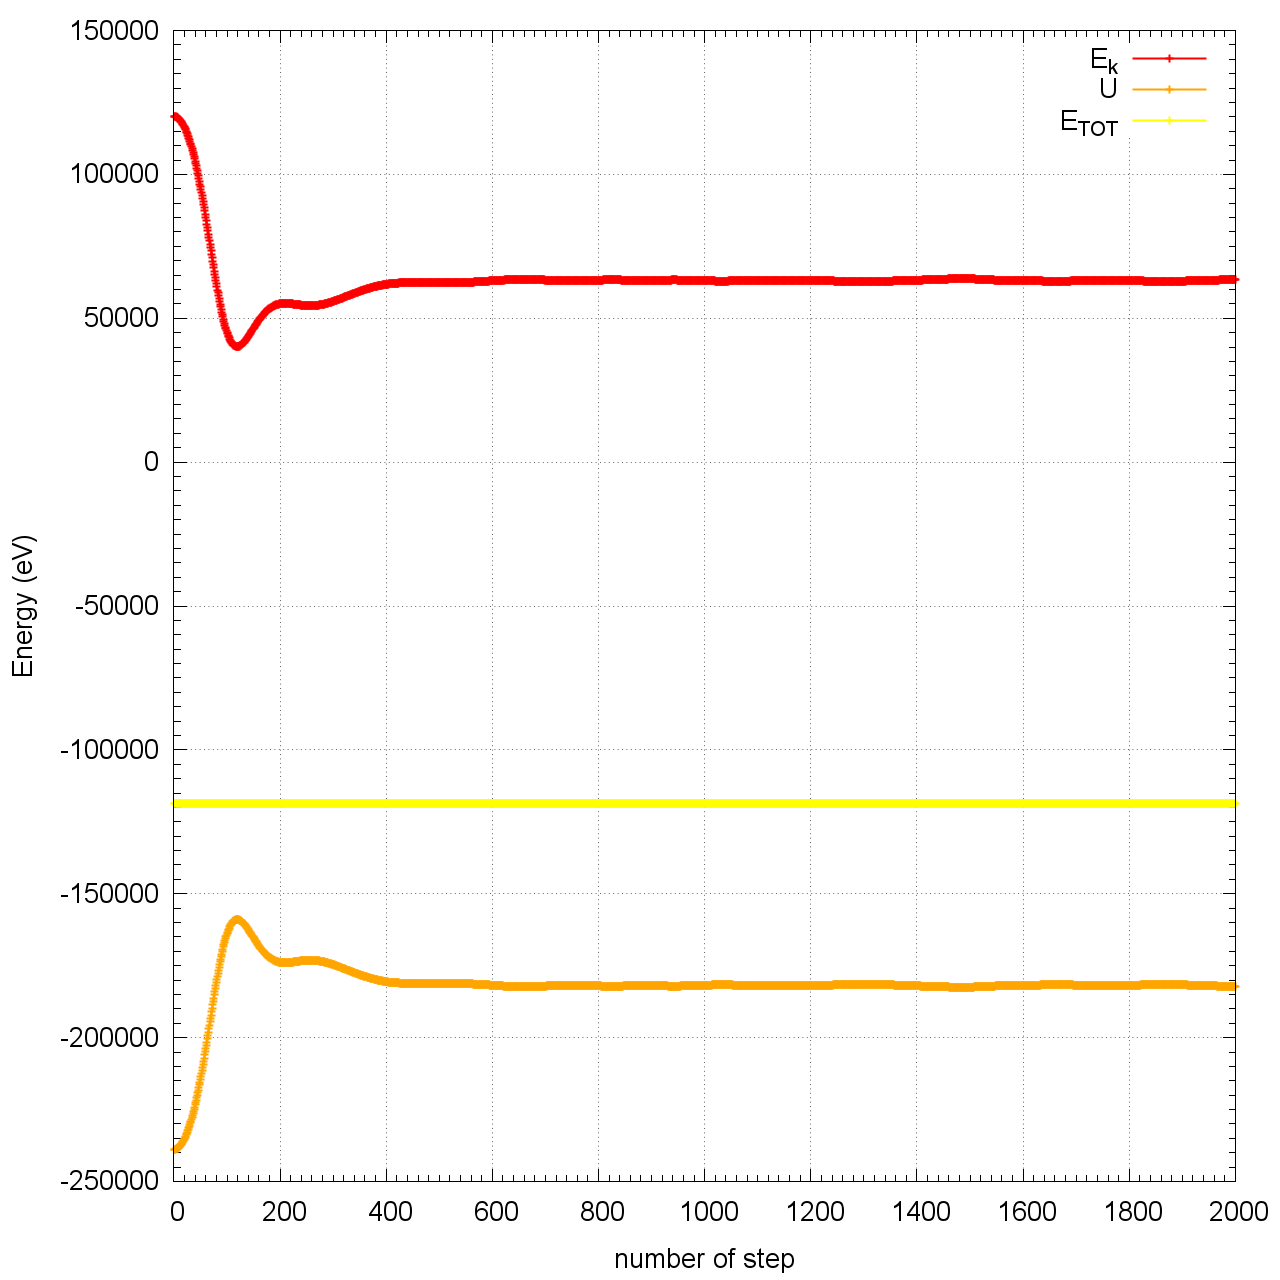
\includegraphics[width=.9\linewidth]{plot_energy_20.png}
  \caption{$E_k$, $E_{pot}$ and $E_{tot}$ over the number of timesteps.}
  \label{fig:sfig2}
\end{subfigure}%
\begin{subfigure}{.5\textwidth}
  \centering
  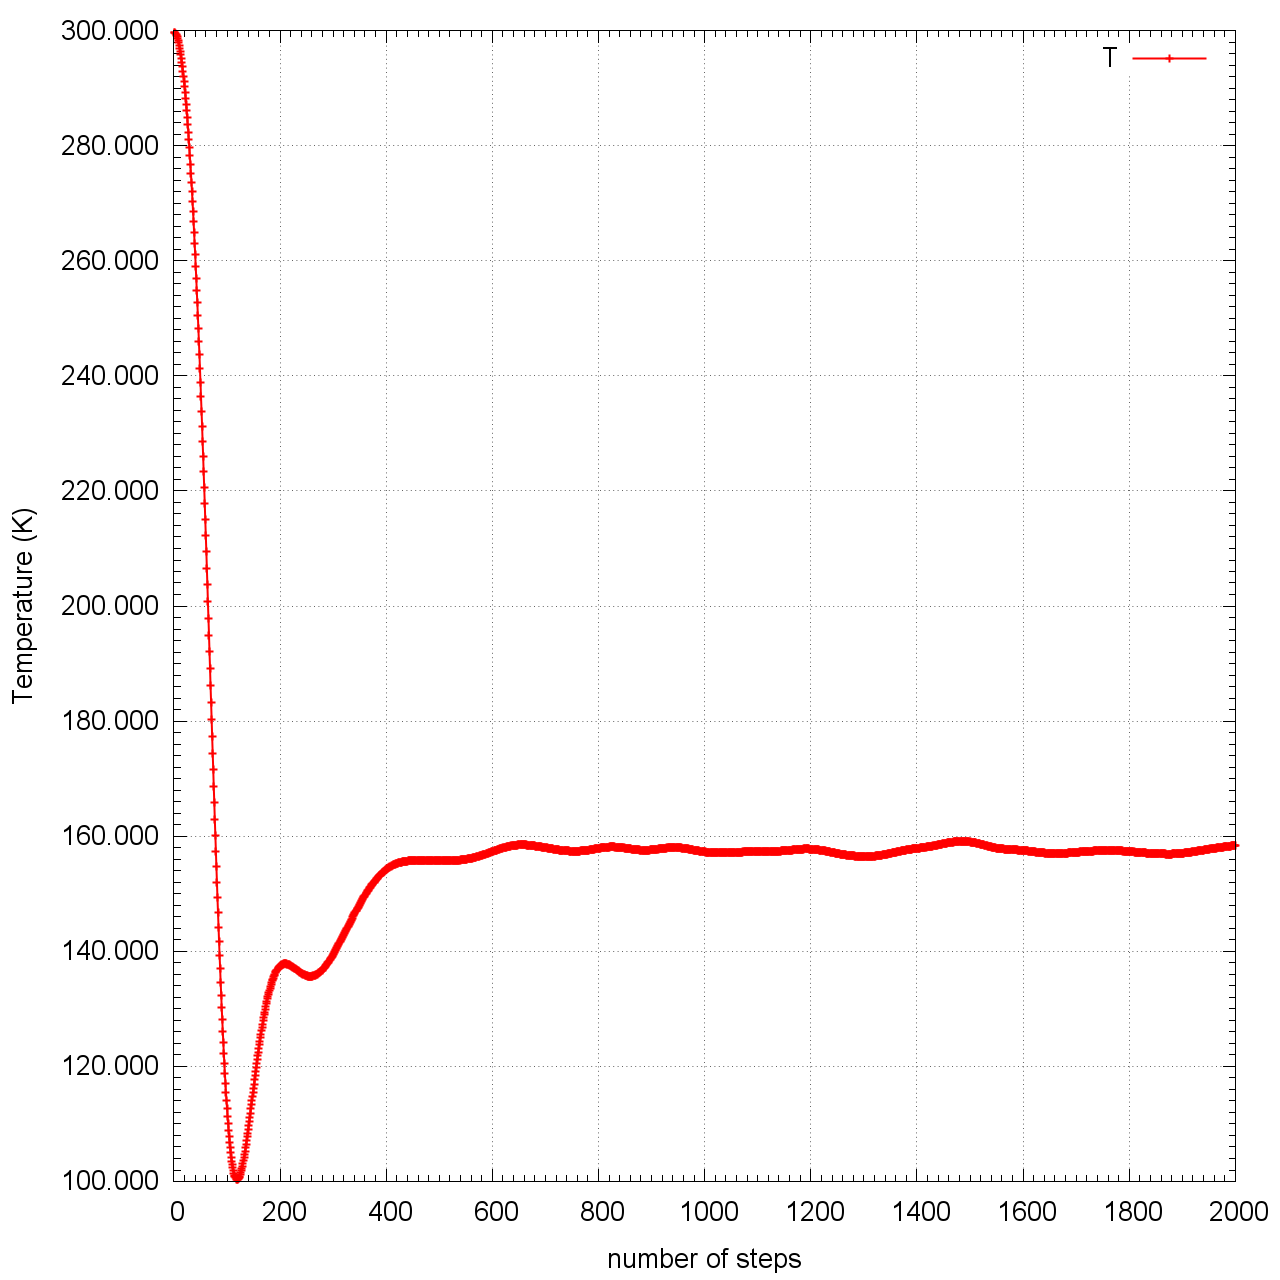
\includegraphics[width=.9\linewidth]{plot_temperature_20.png}
  \caption{\footnotesize Temperature over the number of timesteps.}
  \label{fig:sfig2}
\end{subfigure}%
\caption{{\footnotesize In this case, the bigger number of particles results in a smoother line then before (see fig.5)}}
\label{fig:fig}
\end{figure}
\end{center} 
Exploiting the cell list technique we have managed to simulate even bigger systems, made by $70\times 70 \times 70 \simeq 1.3 \times 10^6$ atoms, which movie simulation can be found at the GitHub address [1].
\begin{center}
\begin{figure}[H]
 \centering
\begin{subfigure}{.5\textwidth}
  \centering
  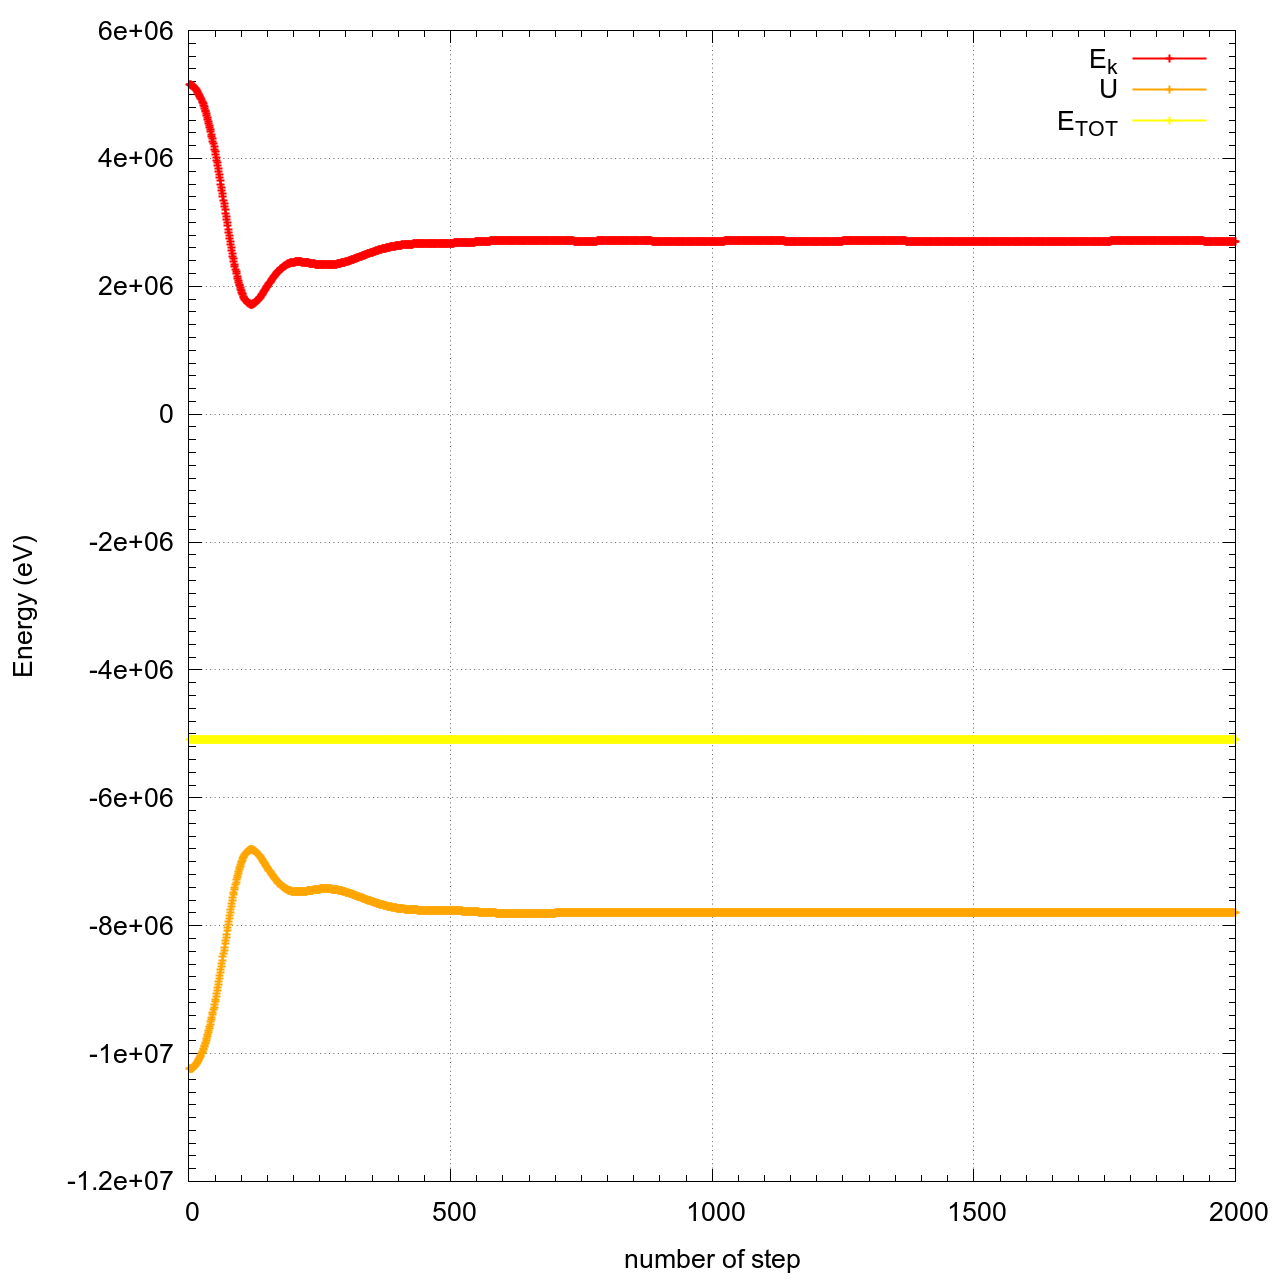
\includegraphics[width=.9\linewidth]{energy70.png}
  \caption{$E_k$, $E_{pot}$ and $E_{tot}$ over the number of timesteps.}
  \label{fig:sfig2}
\end{subfigure}%
\begin{subfigure}{.5\textwidth}
  \centering
  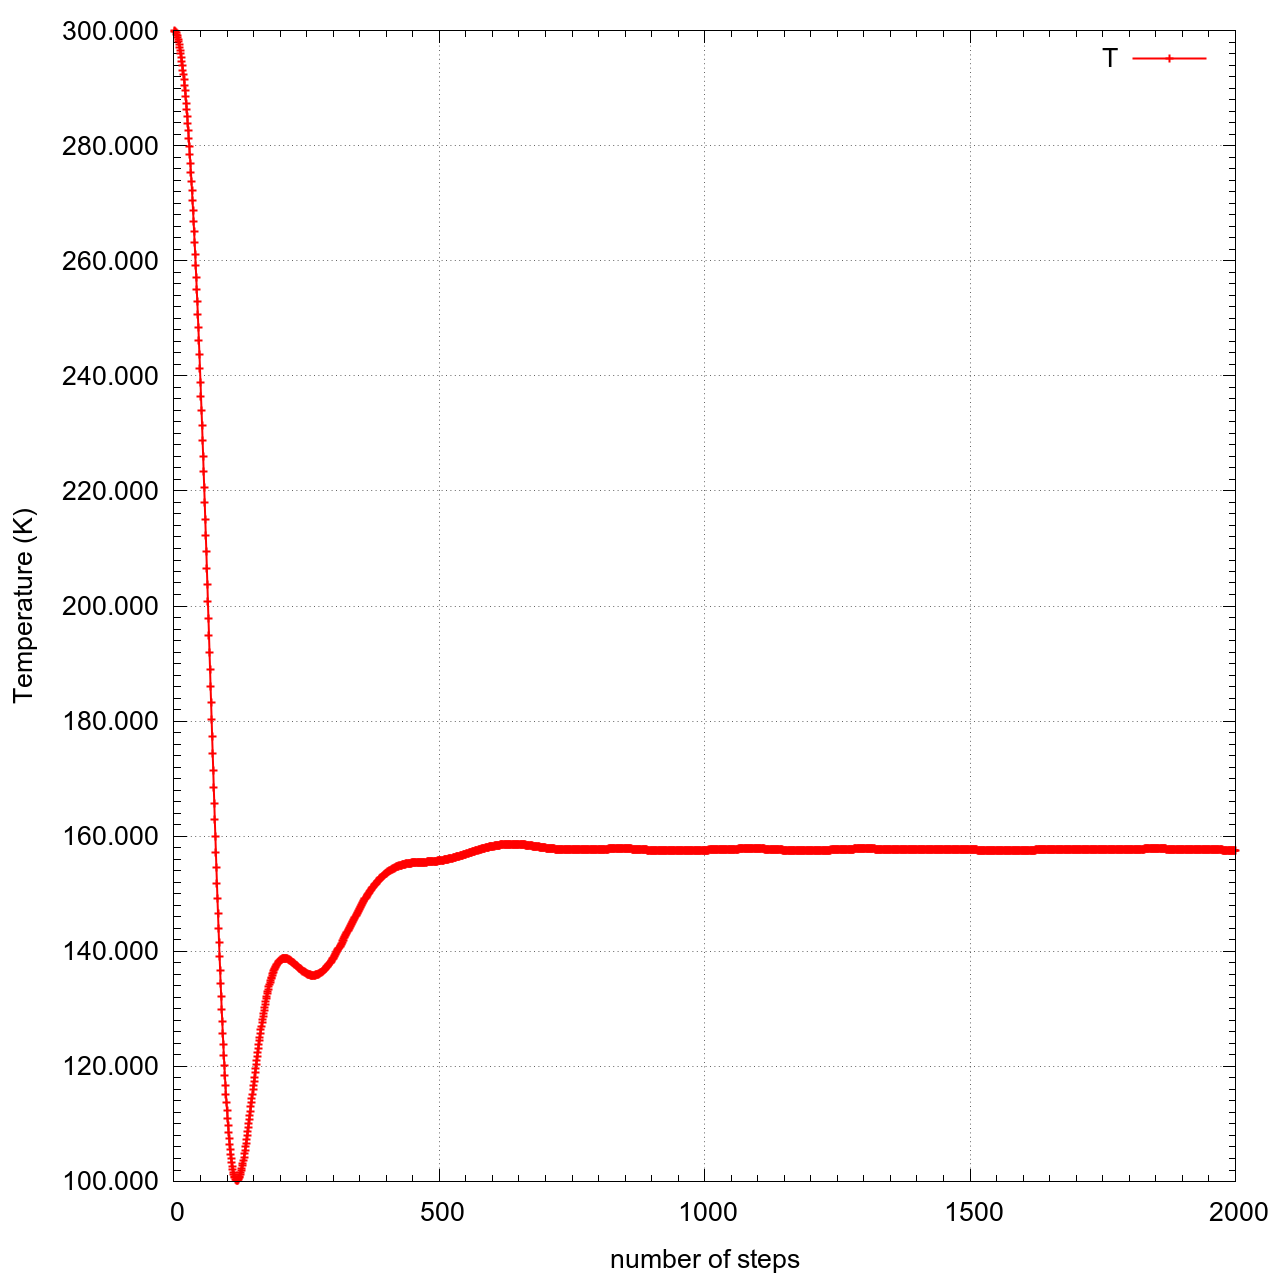
\includegraphics[width=.9\linewidth]{temp70.png}
  \caption{\footnotesize Temperature over the number of timesteps.}
  \label{fig:sfig2}
\end{subfigure}%
\caption{{\footnotesize In this case, the bigger number of particles results in an even smoother line than the previous case}}
\label{fig:fig}
\end{figure}
\end{center} 
We saw that as the number of particles increased we measured more stable final value for the temperature. This
is because it is proportional to the average of the energies of the particles and normally the variance of an average
decreases as the number of elements increases.\\
We have simulated a system made by $4 \times 10^4$
atoms at cold temperature $T = 15K$ and at low density $\rho =
\frac{\rho_c}{125}$ , with
$\rho_c$ the density of the stable crystal structure. We have studied the time evolution of its state for very long time (till
$4 \times 10^5$
time steps, $t_0 = 10^{−15}$s) and we have visualized a condensation of the atoms, as expected, which tend to
agglomerate into droplets from the free initial distribution. A movie simulation of the final time interval $[0.2, 0.4]$[ns]
can be found in the git-hub address [1]. Here some pictures from the simulation:
\begin{center}
\begin{figure}[H]
 \centering
\begin{subfigure}{.34\textwidth}
  \centering
  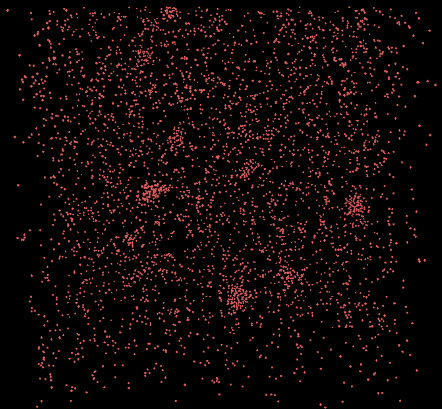
\includegraphics[width=.9\linewidth]{timestep300000.png}
  \caption{After 300000 timesteps.}
  \label{fig:sfiga2}
\end{subfigure}%
\begin{subfigure}{.31\textwidth}
  \centering
  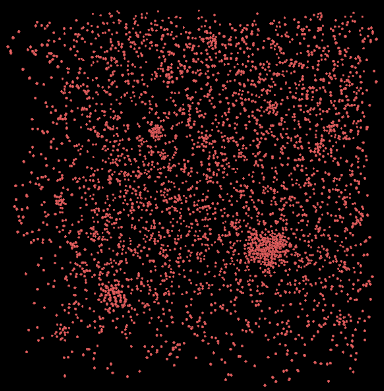
\includegraphics[width=.9\linewidth]{timestep360000.png}
  \caption{After 360000 timesteps}
  \label{fig:sfiga2}
\end{subfigure}%
\begin{subfigure}{.33\textwidth}
  \centering
  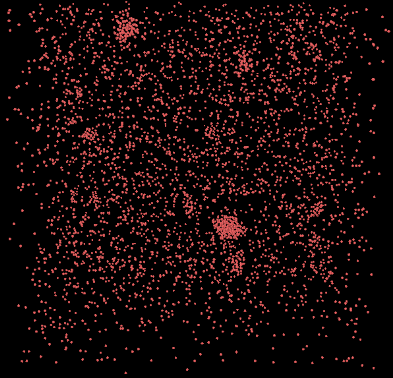
\includegraphics[width=.9\linewidth]{timestep370000.png}
  \caption{After 370000 timesteps}
  \label{fig:sfiga2}
\end{subfigure}%
\caption{{\footnotesize : Here we can see the formation of some droplets at low temperature, low density and longer time simulation
}}
\label{fig:fig}
\end{figure}
\end{center} 


\section*{Thermostat}
\noindent Finally, we implemented a Berendsen thermostat and we ran it to verify its operation. We ran some simulations
with different temperatures and different relaxation times to check its behavior. It was working properly in every
case. Here is a graph with the sampled temperatures over the number of timesteps when the thermostat is on a
temperature of 300 K:

\begin{center}
\begin{figure}[H]
 \centering
\begin{subfigure}{.5\textwidth}
  \centering
  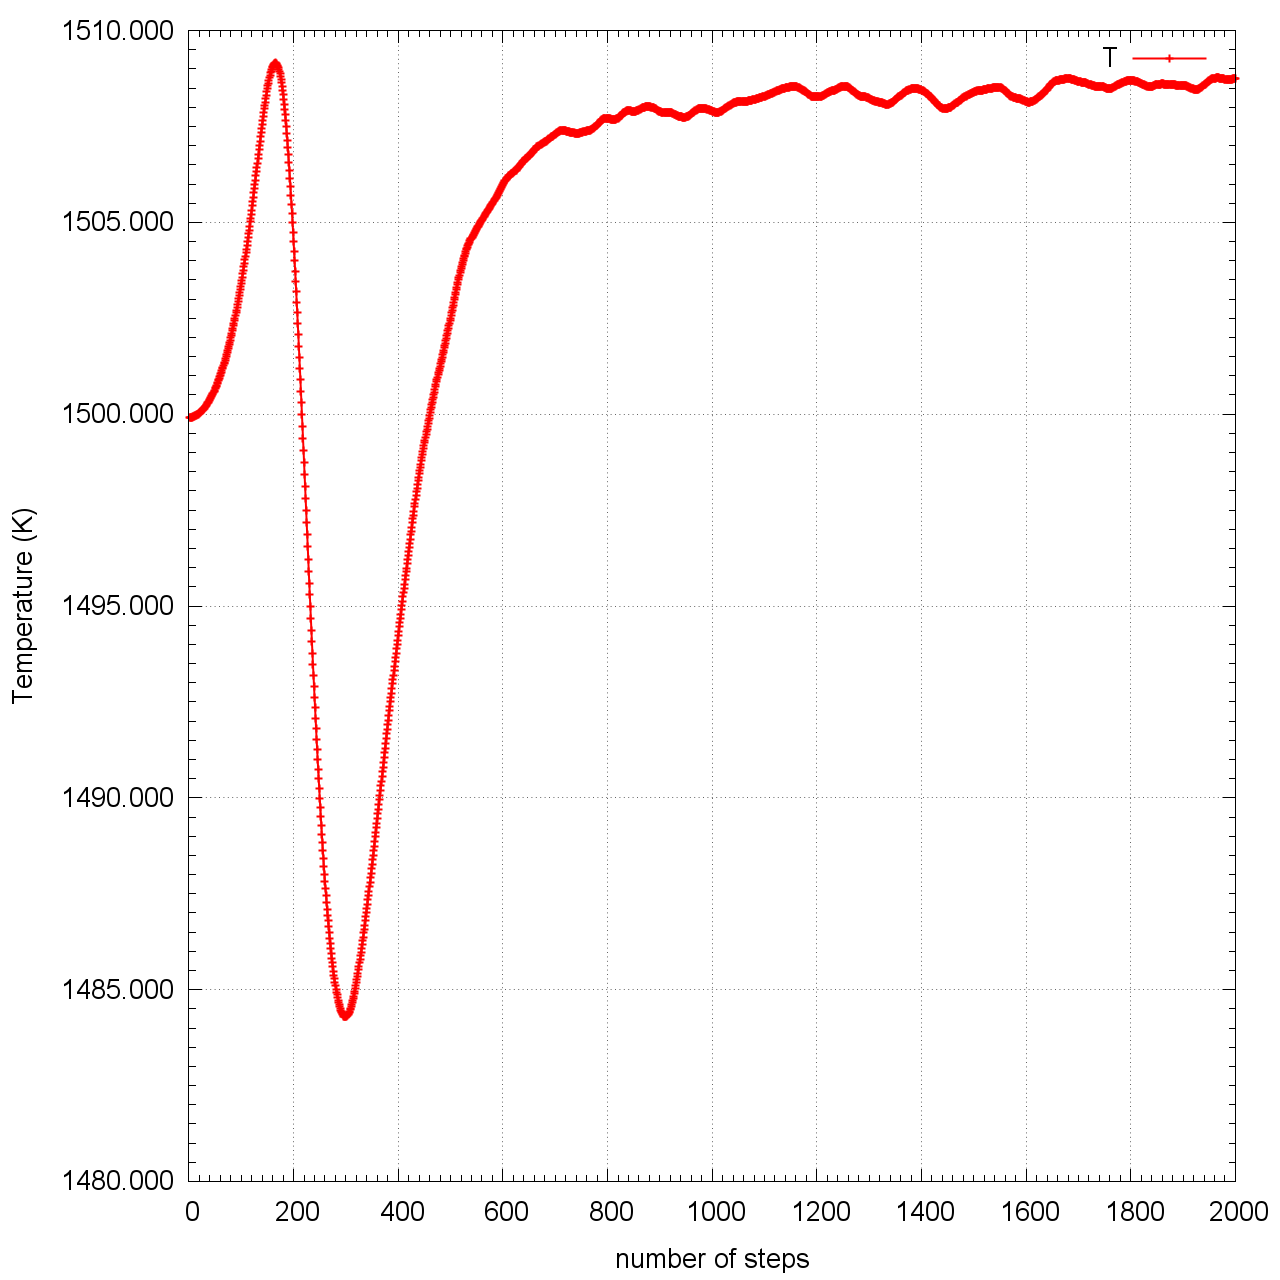
\includegraphics[width=.9\linewidth]{plot_temperature.png}
  \caption{We set the system at a temperature equal to $200K$
while the desired one was $1000K$. The system reaches
the desired temperature after about 800 timesteps
$(8 \times 10^{−13}s)$, then the temperature oscillates around it
within about 5\% of its magnitude.}
  \label{fig:sfig2}
\end{subfigure}%
\begin{subfigure}{.5\textwidth}
  \centering
  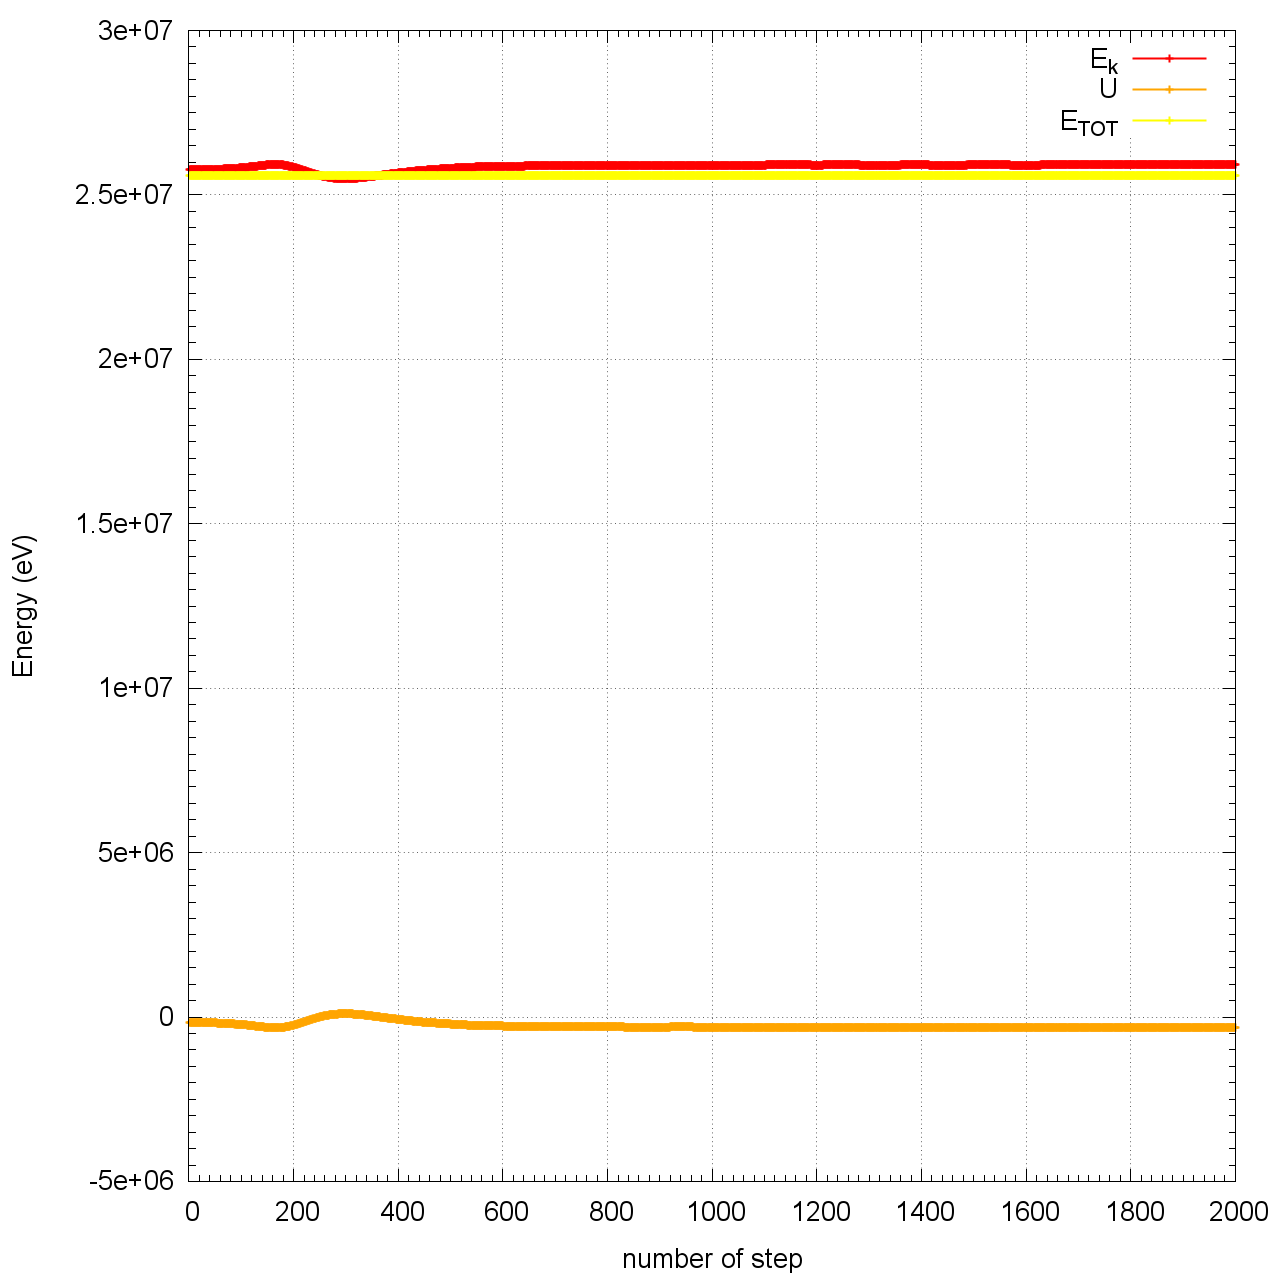
\includegraphics[width=.9\linewidth]{plot_energy.png}
  \caption{\footnotesize Here the kinetic energy, the potential energy and the total energy
are plotted. In this case, of course the total energy isn’t conserved
anymore because the thermostat provides the system with energy}
  \label{fig:sfig2}
\end{subfigure}%

\caption{{\footnotesize The lattice was made of $5\times 5\times 5$ unit cells, so it contained 500 atoms.}}
\label{fig:fig}
\end{figure}
\end{center}

\subsection*{Conclusion} 
\noindent We have implemented a working molecular dynamics program. To be able to simulate bigger lattices, we needed to make our code less CPU consuming. To achieve this, we have started by implementing the cut-off technique to avoid calculations for couples of atoms separated by $5 \sigma$. Then, to simulate even bigger systems, we implemented the cell list algorithm, which allowed us to study lattices made by $\simeq 10^6$ atoms. These simplifications have proven to provide reliable data. As expected, the higher was the number of atoms, the more stable were the sampled values for temperature and potential energy. Our simulation has passed some tests, such as the conservation of total energy and momentum. Comparison between Euler-Cromer and Verlet integrator resulted in the latter being more reliable, as expected.
\\This simulation can be furtherly developed by adding a gravity field and deleting boundary conditions along its direction. In this way the droplets which we observed for small values of pressure would gather at the bottom and the coexistence of gas and liquid phases would be clearer. 
\\Another interesting analysis would have been to plot p-V graphs of an isotherm transformation to show the deviation between the ideal gas equation and van der Waals one; instead of hyperbolas, we would have expected a different shape for low temperatures. To achieve this, it is possible to expand over time the cell size to change the volume of the system. To keep the temperature constant is is possible to exploit Berendsen thermostat.
\subsection*{References}
\noindent $[1]$ Github address : \url {https://github.com/GioPede/FYS3150/tree/master/Project5}
\\ $[2]$ M. Hjort-Jensen. Computational physics, lecture notes fall 2015. Department of Physics, University of Oslo, 2015
\\ $[3]$ $https://en.wikipedia.org/wiki/Moleculardynamics$
\\ $[4]$ $https://en.wikipedia.org/wiki/Argon$
\end{document}